% Standalone vision/pipeline figure: Problem+Challenges -> Ideas+Approach -> Outcome.
% Grayscale only; one line per item; compact spacing; bands drawn with the fit library.
% Compile directly:  pdflatex figures/pipeline_v3.tex  ->  figures/pipeline_v3.pdf
\documentclass[tikz,border=2mm]{standalone}
\usepackage{bm}
\usepackage{amsmath,amssymb}
\usetikzlibrary{positioning,arrows.meta,fit,backgrounds}
\begin{document}
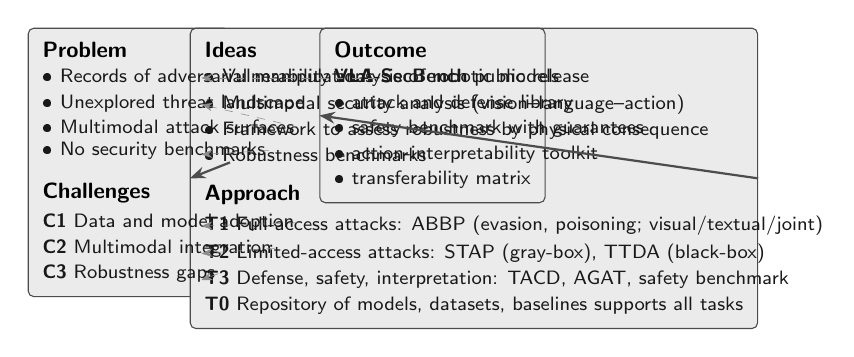
\begin{tikzpicture}[
  font=\footnotesize\sffamily,
  hd/.style={font=\footnotesize\bfseries\sffamily, text=black, inner sep=1pt},
  row/.style={font=\scriptsize\sffamily, text=black!90, anchor=west, inner sep=1pt},
  arr/.style={-{Stealth[length=2mm]}, thick, draw=black!70},
  map/.style={-{Stealth[length=1.4mm]}, very thin, draw=black!45, dashed},
  band/.style={draw=black!70, rounded corners=2pt, fill=black!8, inner sep=4pt},
]
\def\rs{4.6mm} % row spacing

%% ============ Column 1: Problem + Challenges ============
\node[hd] (phd) at (0,0) {Problem};
\node[row, below=0.6mm of phd.south west, anchor=north west] (p1) {\textbullet~Records of adversarial manipulations};
\node[row, below=0.2mm of p1.south west, anchor=north west] (p2) {\textbullet~Unexplored threat landscape};
\node[row, below=0.2mm of p2.south west, anchor=north west] (p3) {\textbullet~Multimodal attack surfaces};
\node[row, below=0.2mm of p3.south west, anchor=north west] (p4) {\textbullet~No security benchmarks};
\node[hd, below=2.2mm of p4.south west, anchor=north west] (chd) {Challenges};
\node[row, below=0.6mm of chd.south west, anchor=north west] (c1) {\textbf{C1} Data and model adoption};
\node[row, below=0.2mm of c1.south west, anchor=north west] (c2) {\textbf{C2} Multimodal integration};
\node[row, below=0.2mm of c2.south west, anchor=north west] (c3) {\textbf{C3} Robustness gaps};

%% ============ Column 2: Ideas + Approach ============
\node[hd, right=9mm of phd] (ihd) {Ideas};
\node[row, below=0.6mm of ihd.south west, anchor=north west] (i1) {\textbullet~Vulnerability analysis of robotic models};
\node[row, below=0.2mm of i1.south west, anchor=north west] (i2) {\textbullet~Multimodal security analysis (vision--language--action)};
\node[row, below=0.2mm of i2.south west, anchor=north west] (i3) {\textbullet~Framework to assess robustness by physical consequence};
\node[row, below=0.2mm of i3.south west, anchor=north west] (i4) {\textbullet~Robustness benchmarks};
\node[hd, below=2.2mm of i4.south west, anchor=north west] (ahd) {Approach};
\node[row, below=0.6mm of ahd.south west, anchor=north west] (t1) {\textbf{T1} Full-access attacks: ABBP (evasion, poisoning; visual/textual/joint)};
\node[row, below=0.2mm of t1.south west, anchor=north west] (t2) {\textbf{T2} Limited-access attacks: STAP (gray-box), TTDA (black-box)};
\node[row, below=0.2mm of t2.south west, anchor=north west] (t3) {\textbf{T3} Defense, safety, interpretation: TACD, AGAT, safety benchmark};
\node[row, below=0.2mm of t3.south west, anchor=north west] (t0) {\textbf{T0} Repository of models, datasets, baselines supports all tasks};

%% ============ Column 3: Outcome ============
\node[hd, right=9mm of ihd] (ohd) {Outcome};
\node[row, below=0.6mm of ohd.south west, anchor=north west] (o0) {\textbf{VLA-SecBench} public release};
\node[row, below=0.2mm of o0.south west, anchor=north west] (o1) {\textbullet~attack and defense library};
\node[row, below=0.2mm of o1.south west, anchor=north west] (o2) {\textbullet~safety benchmark with guarantees};
\node[row, below=0.2mm of o2.south west, anchor=north west] (o3) {\textbullet~action-interpretability toolkit};
\node[row, below=0.2mm of o3.south west, anchor=north west] (o4) {\textbullet~transferability matrix};

%% ============ bands around each column ============
\begin{scope}[on background layer]
  \node[band, fit=(phd)(c3)] (b1) {};
  \node[band, fit=(ihd)(t0)] (b2) {};
  \node[band, fit=(ohd)(o4)] (b3) {};
\end{scope}

%% ============ flows ============
\draw[arr] (b1.east) -- (b2.west);
\draw[arr] (b2.east) -- (b3.west);
% gap-to-idea mappings
\draw[map] (p1.east) -- (i1.west);
\draw[map] (p3.east) -- (i2.west);
\draw[map] (p4.east) -- (i4.west);
% challenge-to-task mappings
\draw[map] (c1.east) -- (t1.west);
\draw[map] (c2.east) -- (t2.west);
\draw[map] (c3.east) -- (t3.west);

\end{tikzpicture}
\end{document}
